%% LyX 2.0.7 created this file.  For more info, see http://www.lyx.org/.
%% Do not edit unless you really know what you are doing.
\documentclass[10pt,twoside,english]{article}
\usepackage{ae,aecompl}
\usepackage{helvet}
\usepackage{courier}
\usepackage[T1]{fontenc}
\usepackage[letterpaper]{geometry}
\geometry{verbose,tmargin=1in,bmargin=1in,lmargin=1in,rmargin=1in}
\setcounter{secnumdepth}{0}
\setcounter{tocdepth}{2}
\usepackage{babel}
\usepackage{varioref}
\usepackage{amsmath}
\usepackage{graphicx}
\usepackage{setspace}
\usepackage{esint}
\onehalfspacing
\usepackage[unicode=true,
 bookmarks=true,bookmarksnumbered=false,bookmarksopen=false,
 breaklinks=false,pdfborder={0 0 0},backref=false,colorlinks=false]
 {hyperref}
\hypersetup{pdftitle={SNPsea: Supplementary Text},
 pdfauthor={Kamil Slowikowski}}

\makeatletter

%%%%%%%%%%%%%%%%%%%%%%%%%%%%%% LyX specific LaTeX commands.
%% Because html converters don't know tabularnewline
\providecommand{\tabularnewline}{\\}

\AtBeginDocument{
  \def\labelitemi{\(\cdot\)}
}

\makeatother

\begin{document}

\title{SNPsea: an algorithm to identify cell types, tissues, and pathways
affected by risk loci}


\author{Kamil Slowikowski, Xinli Hu, Soumya Raychaudhuri}

\maketitle
\tableofcontents{}

\newpage{}


\section{Supplementary Note}


\subsection{Algorithm Details}

SNPsea tests if genes implicated by risk loci (e.g., those discovered
through genome-wide association (GWA) studies) are specifically expressed
in some conditions over others, and if this specificity is statistically
significant. The program requires two inputs:
\begin{enumerate}
\item A list of SNP identifiers: rs123, 12:456, ...
\item A matrix of genes and conditions, such as:

\begin{itemize}
\item expression profiles of different cell types.
\item Ontology terms and presence/absence 1/0 values for each gene in each
term.
\end{itemize}
\end{enumerate}
For example, SNPsea can be used to find tissues or cell types whose
function is likely to be influenced by genes in risk loci. If the
genes in risk loci are used in relatively few cell types, we hypothesize
that they are likely to affect those cell types' unique functions.
This assumes that expression specificity is a good indicator of a
gene's importance to the unique function of the cell type.

For a given set of SNPs associated to some phenotype, SNPsea tests
whether all implicated genes, in aggregate, are enriched for specificity
to a condition in a user-provided matrix of genes and conditions/annotations.
The algorithm consists of three steps:
\begin{itemize}
\item \textbf{Step 1: Assigning genes to each SNP}

\begin{itemize}
\item We use linkage disequilibrium (LD) to identify the genes implicated
by each SNP.
\end{itemize}
\item \textbf{Step 2: Calculating specificity scores}

\begin{itemize}
\item We look up implicated genes in a user-provided matrix and calculate
a specificity score for each annotation/condition based on the values
of these genes.
\end{itemize}
\item \textbf{Step 3: Testing significance}

\begin{itemize}
\item We compare the specificity scores to a null distribution of scores
obtained with random sets of matched SNP sets and compute an empirical
$P$-value. 
\end{itemize}
\end{itemize}

\subsubsection*{Step 1: Assigning genes to each SNP}

Accurate analyses must address the critical issue that SNPs frequently
implicate a region with multiple different genes (\textbf{Supplementary
Figure 2}). The challenge is to find evidence to show which of those
genes are associated with a given trait.

We determine the genes plausibly implicated by each trait-associated
SNP using a previously described strategy (\textbf{Supplementary Figure
1} and \cite{rossin_proteins_2011}). First, we define the linkage
interval for a given SNP as the span between the furthest correlated
SNPs $r^{2}>0.5$ (EUR) within a 1 Mb window \cite{consortium_integrated_2012}.
Next, we extend the interval to the nearest recombination hotspots
with recombination rate >3 cM/Mb \cite{myers_fine-scale_2005}. To
address the case when no genes overlap an interval, we provide an
option for SNPsea to extend the interval up- and downstream (by default
10 Kb).

Most frequently, we find multiple genes $(m_{k}>1)$ in a single SNP
locus $k$. We expect many loci with multiple genes because of regions
with high LD across long stretches of a chromosome. Less frequently,
a locus has a single gene $(m_{k}=1)$, and loci with no genes $(m_{k}=0)$
are discarded.

After each SNP has been assigned an interval and a set of genes overlapping
the interval, we merge SNPs with shared genes into a single locus
to avoid multiple-counting of genes.


\subsubsection*{Step 2: Calculating specificity scores}

SNPsea uses different algorithms for matrices with continuous or binary
values. By default, SNPsea assumes one gene in each associated locus
is associated with the given trait. We also include the option to
assume all genes within a locus are associated. We compare results
of the two options with four phenotypes (\textbf{Supplementary Figure
4}). \label{par:single_total}
\begin{enumerate}
\item The \texttt{'-{}-score single'} option (default) assumes that a single
gene in each locus is associated with the given phenotype. For each
condition, we choose the gene in each locus with the greatest specificity
to that condition.
\item The \texttt{'-{}-score total'} option assumes that all genes in a
SNP's linkage interval are associated. We account for all linked genes
when calculating scores.
\end{enumerate}

\paragraph{Specificity for a matrix of continuous values}

Before running SNPsea, a matrix with continuous values must be normalized
so that columns are directly comparable. \emph{It is not appropriate
to use this method on a ``raw'' matrix of expression values}.

We extend an approach we have previously described in detail \cite{hu_integrating_2011}.
Let $A$ denote a continuous gene expression matrix with $m$ genes
and $n$ conditions. First, we normalize the expression of each gene
by dividing each value by the L2 norm of the gene's values across
all conditions.

\[
A'_{i,j}=\dfrac{A_{i,j}}{\sqrt{A_{i,1}^{2}+A_{i,2}^{2}+\cdots+A_{i,n}^{2}}}
\]


The resulting matrix $A'$ has values $A'_{i,j}$ between 0 and 1
indicating specificity of gene $i$ to condition $j$. A value $A'_{i,j}=1$
indicates that gene $i$ is exclusively expressed in condition $j$,
and $A'_{i,j}=0$ indicates that gene $i$ is not expressed in condition
$j$.

Next, we transform $A'$ to a matrix $A''$ of non-parametric condition-specificity
percentiles as follows. For each condition $j$, we rank the values
of $A'_{,j}$ in ascending order and divide them by the number of
genes $m$, resulting in percentiles between 0 and 1 where a lower
value indicates greater specificity to the given condition.

\[
A''_{i,j}=\dfrac{\text{Rank}_{j}(A'_{i,j})}{m}
\]


\medskip{}



\paragraph*{Locus scores for a matrix of continuous values}

We create a new matrix $P$, where each value $P_{k,j}$ is a score
for a SNP locus $k$ and a condition $j$. We define the locus scores
$P_{,j}$ for a single condition $j$ to be approximately uniformly
distributed for a set of randomly selected loci under the null hypothesis
of no association to the condition. We make the assumption that, for
a set of genes in a given SNP locus $I_{k}$, the values $A''_{i\in I_{k},j}$
are random, independent, and approximately uniformly distributed.
If there is an actual association to a condition $j$, we will observe
an unexpectedly small value for $P_{,j}$.


\paragraph*{\texttt{'-{}-score single' (default)}}

This approach tests for the association of one gene in each SNP locus
to condition $j$.

For each locus-condition pair $(k,j)$, we choose the single gene
$i$ in locus $k$ with greatest specificity to condition $j$ among
the $m_{k}$ genes in the locus, as previously described in Hu \emph{et
al.} \cite{hu_integrating_2011}. Let $g_{k}$ denote this most specific
gene, so that $A''_{g_{k},j}=\text{Min}_{i\in I_{k}}(A''_{i,j})$
where $I_{k}$ denotes the set of genes in locus $k$. If we assume
values of $A''_{i\in I_{k},j}$ are uniformly distributed for a given
condition $j$ and genes $i\in I_{k}$, then the probability to randomly
draw a value equal to or less than $A''_{g_{k},j}$ is as follows:

\[
P_{k,j}=1-(1-\text{Min}_{i\in I_{k}}(A''_{i,j}))^{m_{k}}
\]



\paragraph*{\texttt{'-{}-score total'}}

This approach tests for the association of all genes in each SNP locus
to condition $j$ --- we consider this model to be unlikely in most
situations. The product (log sum) of uniform values between (0,1)
follows a gamma distribution \cite{johnson_univariate_2005}. If the
genes $I_{k}$ have no specificity to a condition $j$, then the values
$A''_{i\in I_{k}}$ are approximately uniformly distributed. So, we
compute the probability to randomly draw values $A''_{i\in I_{k}}$
with a smaller product as the upper tail of the gamma distribution:

\begin{eqnarray*}
P_{k,j} & = & \int_{x}^{\infty}\Gamma(m_{k},1)\ \ \text{for}\ \ x=\sum_{i\in I_{k}}-\text{ln}A''_{i,j}
\end{eqnarray*}


\medskip{}



\paragraph*{Locus scores for a matrix of binary values}

Let $B$ denote a binary matrix (1=present, 0=absent) with $m$ genes
and $n$ conditions. Let $m_{j}$ denote the number of genes present
in condition $j$. Let $m_{k}$ denote the number of genes in locus
$k$ and $m_{k,j}\le m_{k}$ denote the number of genes in locus $k$
that are present in condition $j$.

We provide two options to calculate locus scores. By default, we account
for presence or absence of any of the $m_{k}$ genes in condition
$j$, as shown below (\texttt{'-{}-score single'}). Alternatively,
we account for the number of genes in a given locus (\texttt{'-{}-score
total'}).

\medskip{}


\hspace*{\fill}%
\begin{tabular}{ccccccc}
 &  &  & \texttt{'-{}-score single'} &  &  & \texttt{'-{}-score total'}\tabularnewline
\noalign{\vskip2mm}
$p(x)=\dfrac{{m_{j} \choose x}{m-m_{j} \choose m_{k}-x}}{{m \choose m_{k}}}$ &  &  & $P_{k,j}=\begin{cases}
1-p(0) & m_{k,j}>0\\
1 & m_{k,j}=0
\end{cases}$ &  &  & $P_{k,j}=\begin{cases}
1-\sum_{x=0}^{m_{k,j}-1}p(x) & m_{k,j}>0\\
1 & m_{k,j}=0
\end{cases}$\tabularnewline
\end{tabular}\hspace*{\fill}

\medskip{}



\paragraph*{Condition specificity scores}

For both continuous and binary matrices, we define a specificity score
$S_{j}$ for each condition $j$ as the aggregate of $P_{k,j}$ values
across SNP loci:

\[
S_{j}=\sum_{k}-\text{log}P_{k,j}
\]



\subsubsection*{Step 3: Testing significance }


\paragraph{Analytical p-values}

We previously found that aggregating the $P_{k,j}$ scores and determining
a $P$-value analytically from a distribution results in inaccurate
p-values \cite{hu_integrating_2011}. $A''_{i,j}$ values may be relatively
uniform genome-wide, but proximate genes often have shared functions.
The genome has a complex correlation structure of linkage disequilibrium,
gene density, gene size and function that is challenging to model
analytically. We use the sampling strategy described below instead.


\paragraph{Permutation p-values}

For each condition, we use a sampling approach to calculate an empirical
p-value. This is the tail probability of observing a condition-specificity
score greater or equal to $S_{j}$. We obtain the distribution empirically
with null SNP sets.

We compute specificity scores $S$ for random SNP sets. Each SNP in
a null set is matched to a SNP in the user's set on the number of
linked genes. To adequately sample genes from the entire genome, we
sample SNP sets from a list of LD-pruned SNPs (subset of SNPs in 1000
Genomes Project) \cite{lango_allen_hundreds_2010}.

For each condition $j$, we calculate an exact permutation p-value
\cite{phipson_permutation_2010}. Let $a_{j}$ denote the number of
sampled SNP sets (e.g. 10,000) and let $b_{j}$ denote how many null
specificity scores are greater than or equal to the user's score $S_{j}$:

\[
p_{j}=\dfrac{b_{j}+1}{a_{j}+1}
\]


We implemented adaptive sampling to calculate p-values efficiently.
As each condition is tested for significance, we increase the number
of iterations to resolve significant p-values and save computation
by using fewer iterations for less significant p-values. Two options
allow the user to control the adaptive sampling:
\begin{enumerate}
\item \texttt{'-{}-max-iterations N'} The maximum number of iterations for
each condition. We stop testing a condition after sampling $N$ SNP
sets.
\item \texttt{'-{}-min-observations N'} The minimum number of observed null
specificity scores greater than or equal to $S_{j}$ required to stop
sampling SNP sets for a condition $j$.
\end{enumerate}

\subsection{Data}

Please find the data required to reproduce this analysis here: \href{http://dx.doi.org/10.6084/m9.figshare.871430}{http://dx.doi.org/10.6084/m9.figshare.871430}


\subsubsection*{Gene Atlas gene expression matrix}

We downloaded the data from BioGPS: \href{http://plugins.biogps.org/download/gnf1h-gcrma.zip}{http://plugins.biogps.org/download/gnf1h-gcrma.zip}

We averaged the expression values for tissue replicates. For each
gene, we selected the single probe with the largest minimum value.
Finally, we converted the file to \href{http://www.broadinstitute.org/cancer/software/genepattern/gp_guides/file-formats/sections/gct}{GCT format}.


\subsubsection*{Gene Ontology binary presence/absence matrix}

We downloaded the OBO file from Gene Ontology (data-version: 2013-06-29,
CVS revision: 9700):

\href{http://www.geneontology.org}{http://www.geneontology.org}

For each gene, we climbed the hierarchy of ontology terms and applied
parental terms. If a gene is annotated with some term $T$, we also
add all of the terms that are parents of $T$. We copy terms between
homologous genes using Homologene data (\href{http://www.ncbi.nlm.nih.gov/homologene}{http://www.ncbi.nlm.nih.gov/homologene}).
If a mouse gene is annotated with some term and the human homolog
is not, then we copy the term to the human gene. We discard all GO
terms assigned to fewer than 100 or to more than 1000 genes. This
leaves us with a matrix of 19,111 genes and 1,751 terms.


\subsubsection*{1000 Genomes Project}

We downloaded a filtered (diallelic and 5 or more copies of the minor
allele) set of markers from the BEAGLE website and calculated pairwise
LD (EUR) for all SNPs in a 1 Mb sliding window: 

\href{http://bochet.gcc.biostat.washington.edu/beagle}{http://bochet.gcc.biostat.washington.edu/beagle}


\subsection{Commands}

More details:\textbf{\large{} \href{http://www.broadinstitute.org/mpg/snpsea/SNPsea_manual.html}{http://www.broadinstitute.org/mpg/snpsea/SNPsea\_{}manual.html}}{\large \par}

\begin{tabular}{cc}
Analysis & Figures\tabularnewline
\hline 
\texttt{\small{}}%
\begin{tabular}{c}
\tabularnewline
\texttt{\small{}}%
\begin{minipage}[t]{0.5\columnwidth}%
\texttt{\small{}snpsea}{\small \par}

\texttt{\small{}-{}-snps HDL\_Teslovich2010.txt}{\small \par}

\texttt{\small{}-{}-gene-matrix GeneAtlas2004.gct.gz}{\small \par}

\texttt{\small{}-{}-gene-intervals NCBIgenes2013.bed.gz}{\small \par}

\texttt{\small{}-{}-snp-intervals TGP2011.bed.gz}{\small \par}

\texttt{\small{}-{}-null-snps Lango2010.txt.gz}{\small \par}

\texttt{\small{}-{}-score single}{\small \par}

\texttt{\small{}-{}-out <out>}{\small \par}

\texttt{\small{}-{}-slop 10e3}{\small \par}

\texttt{\small{}-{}-threads 2}{\small \par}

\texttt{\small{}-{}-null-snpsets 0}{\small \par}

\texttt{\small{}-{}-min-observations 100}{\small \par}

\texttt{\small{}-{}-max-iterations 1e6}%
\end{minipage}\tabularnewline
\end{tabular} & %
\begin{tabular}{l}
Horizontal bar plot of p-values:\tabularnewline
\texttt{\small{}snpsea-barplot <out>}\tabularnewline
\tabularnewline
Heatmap of conditions and loci:\tabularnewline
\texttt{\small{}snpsea-heatmap <out>}\tabularnewline
\tabularnewline
Type 1 error rates for each condition:\tabularnewline
\texttt{\small{}snpsea-type1error <out>}\tabularnewline
\end{tabular}\tabularnewline
\end{tabular}

\newpage{}


\section{Supplementary Figures}


\subsection{Supplementary Figure 1: Determining SNP linkage intervals}

\hfill{}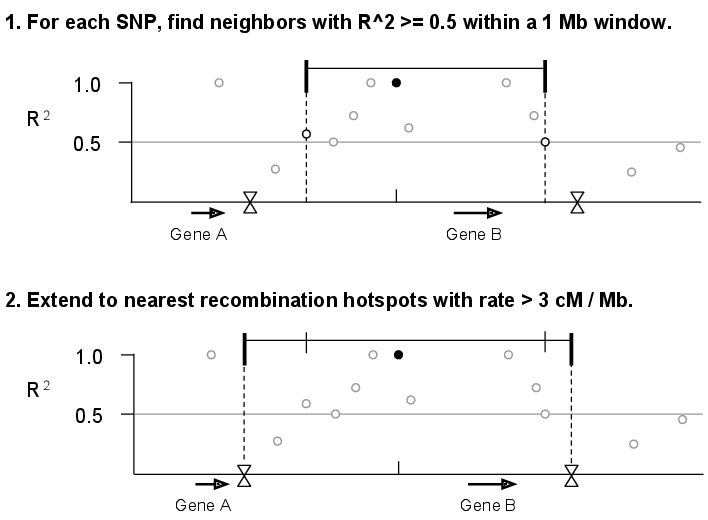
\includegraphics[width=0.75\textwidth]{figures/snp_linkage_intervals}\hfill{}

We calculated $r^{2}$ values for all pairs of SNPs within a 1 Mb
sliding window along each chromosome. Next, we assigned each of the
SNPs from The 1000 Genomes Project Phase I \cite{consortium_integrated_2012}
to a linkage interval by identifying each SNP's furthest upstream
and downstream neighbors with $r^{2}\ge0.5$. Finally, we extended
each interval to recombination hotspots reported by HapMap \cite{myers_fine-scale_2005}
with recombination rate >3 cM/Mb.

\newpage{}


\subsection{Supplementary Figure 2: Counting genes in GWAS SNP linkage intervals}

\hfill{}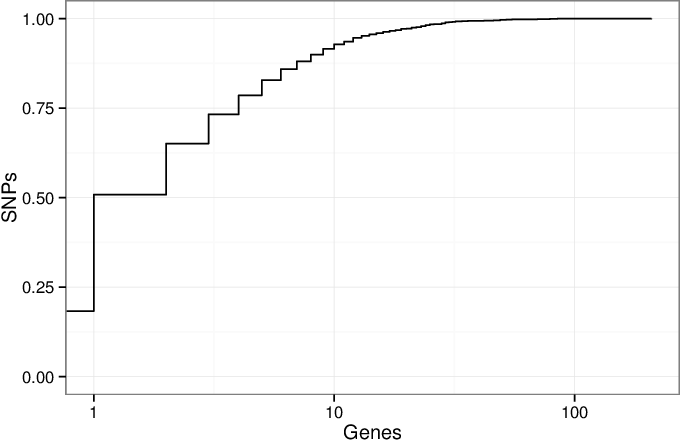
\includegraphics[width=0.75\textwidth]{figures/gwas_ngenes}\hfill{}

A cumulative density plot of the number of genes overlapped by the
linkage intervals of GWAS SNPs. We downloaded the GWAS Catalog SNPs
on January 17, 2014 and selected the 11,561 SNPs present in the 1000
Genomes Project \cite{consortium_integrated_2012}. Of these SNPs,
2,119 (18\%) of them have linkage disequilibrium (LD) intervals that
overlap no genes, and 3,756 (32\%) overlap a single gene. The remaining
50\% of SNPs overlap 2 or more genes. This illustrates the critical
issue that many SNPs implicate more than one gene.

\newpage{}


\subsection{Supplementary Figure 3: Choosing the $r^{2}$ threshold for linkage
intervals}

\hfill{}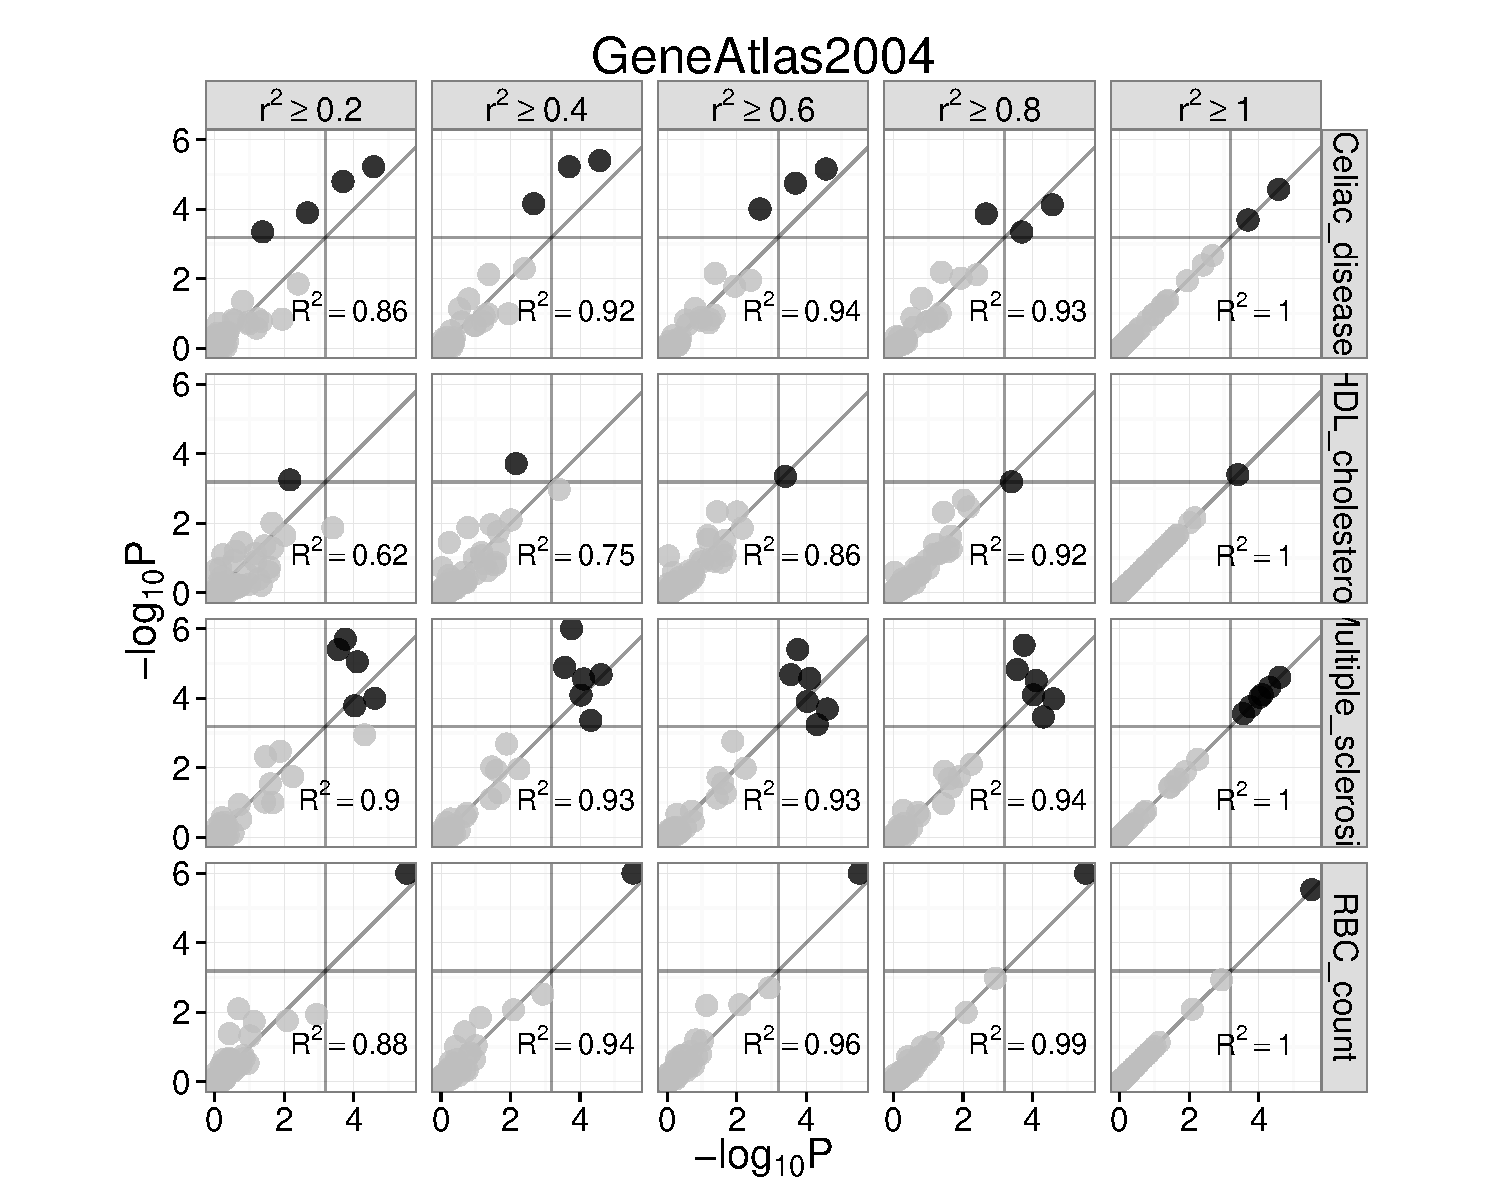
\includegraphics[width=0.6\textwidth]{figures/r2_thresholds-GeneAtlas2004}\hfill{}

\hfill{}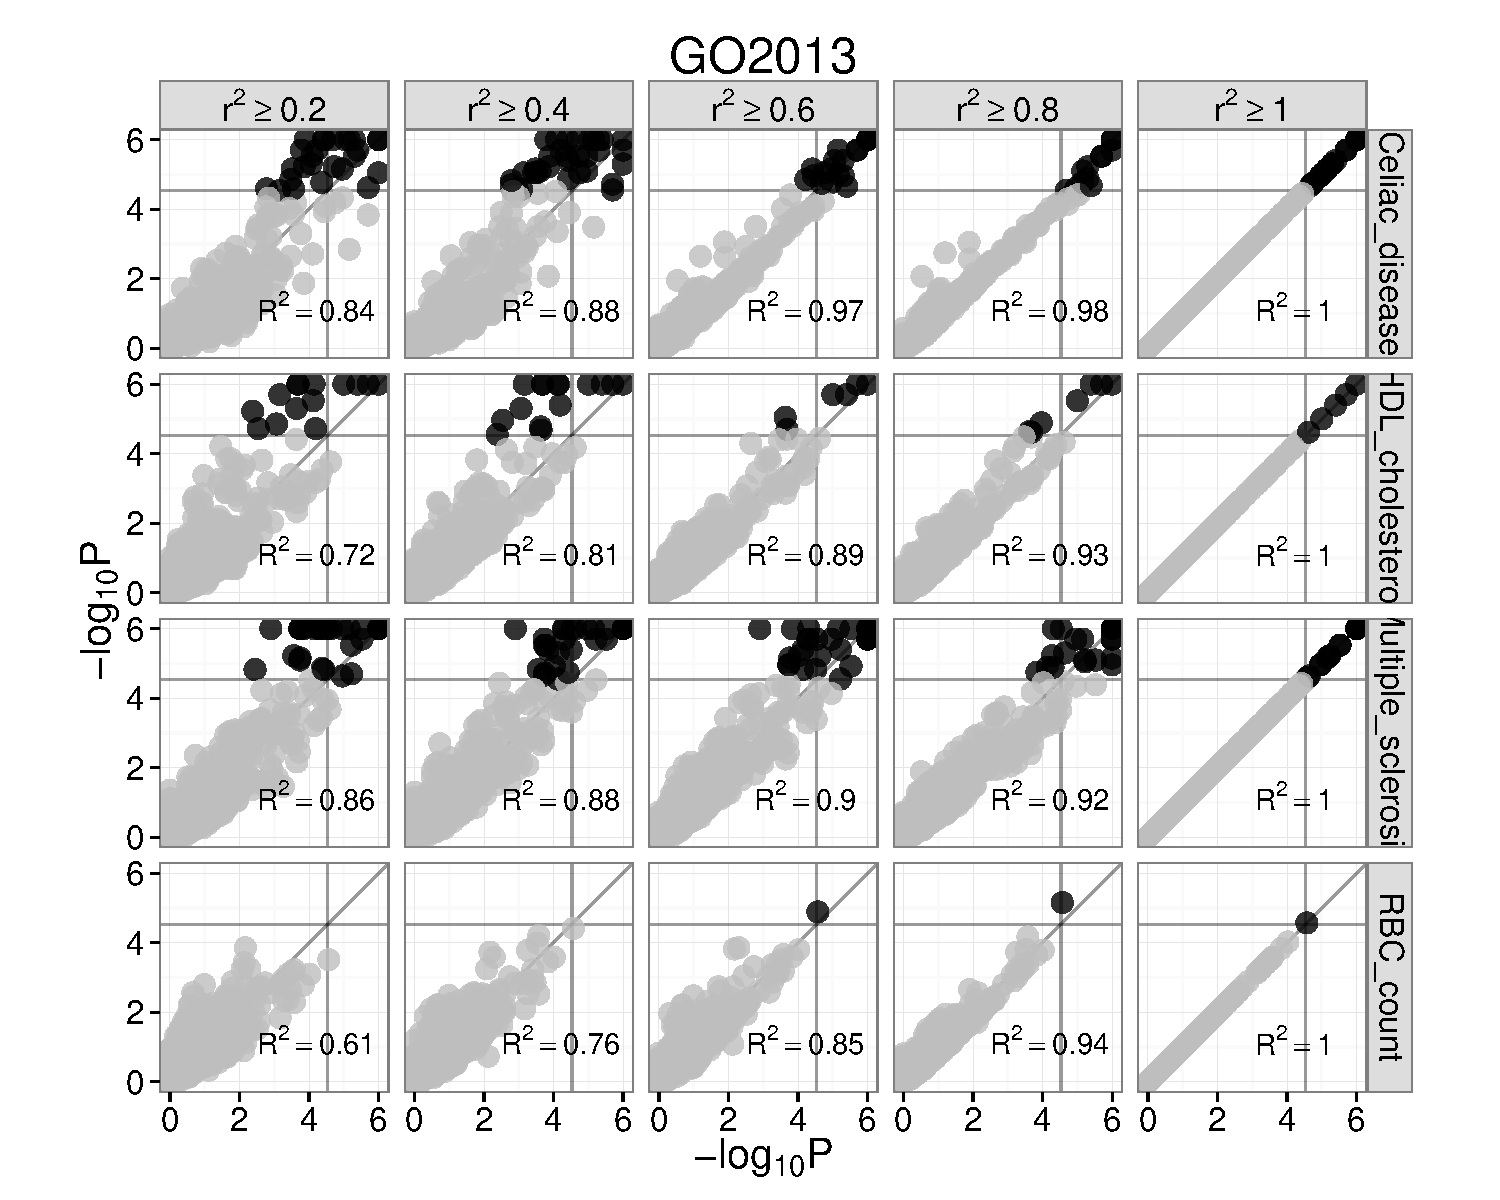
\includegraphics[width=0.6\textwidth]{figures/r2_thresholds-GO2013}\hfill{}

Gene Atlas and Gene Ontology (top and bottom). Each subplot has $-\text{log}_{10}P$
for $r^{2}=1$ on the x-axis and $-\text{log}_{10}P$ on the y-axis
for the $r^{2}$ threshold marked above. Grey lines are significance
thresholds after correction testi threshold marked above. Grey lines are significance
thresholds after correction testing multiple conditions (cell types,
GO annotations). Black points are significant and grey are not. We
used the \texttt{'-{}-score single'} option. Red blood cell count
SNPs are enriche$r^{2}=(0.6,0.8,1.0)$. This result falls
below the multiple testing threshold at $r^{2}\ge0.4$, but remains. This result falls
below the (see main text).

To investigate if the choice of $r^{2}$ threshold influences SNPsea
results, we repeated the analysis of four traits using 5  threshold influences SNPsea
res 0.2, 0.4, 0.6, 0.8, 1.0). SNPsea results seem
to be robust to the choice of threshold 0.2, 0.4, 0.6, 0.8, 1.0). SNPsea results seem
to be robust to the choice of threshold, mostly due to the fact that
we extend linkage intervals for each SNP to the nearest recombination
ho for our analysis and for our provided data
files due to this result, and also due to  for our analysis and for our provided data
files due to thi


\subsection{Supplementary Figure 4: Comparison of 'single' and 'total' options}

\h


\su\includegraphics[width=1\textwidth]{figures/single_vs_total-RBC-MS-CD-HDL}\hfill{}

Qu\includegraphics[width=1\textwidth]{/home/kamil/work/snpsea/doc/figures/single_vs_total-RBC-MS-CD-HDL.png}\hfill{}

Quantile-quantile plots for Gene Atlas \cite{su_gene_2004} and Gene
Ontology (top and bottom). The x and y axes are $-\text{log}_{10}P$
for \texttt{'-{}-score single' and '-{}-score total'} SNPsea options,
respectively. The \texttt{'single'} and \texttt{'total'} methods are
described \vpageref{par:single_total}. The $P$-value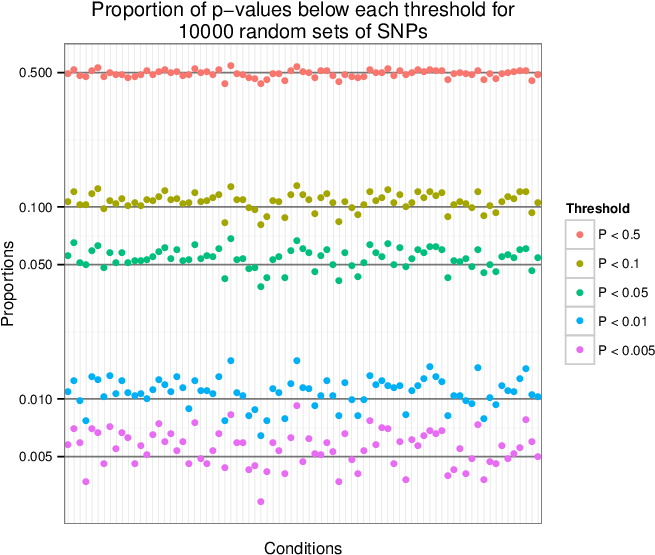
\includegraphics[width=0.65\textwidth]{figures/type1error_GeneAtlas2004}\hfill{}

\hfill{}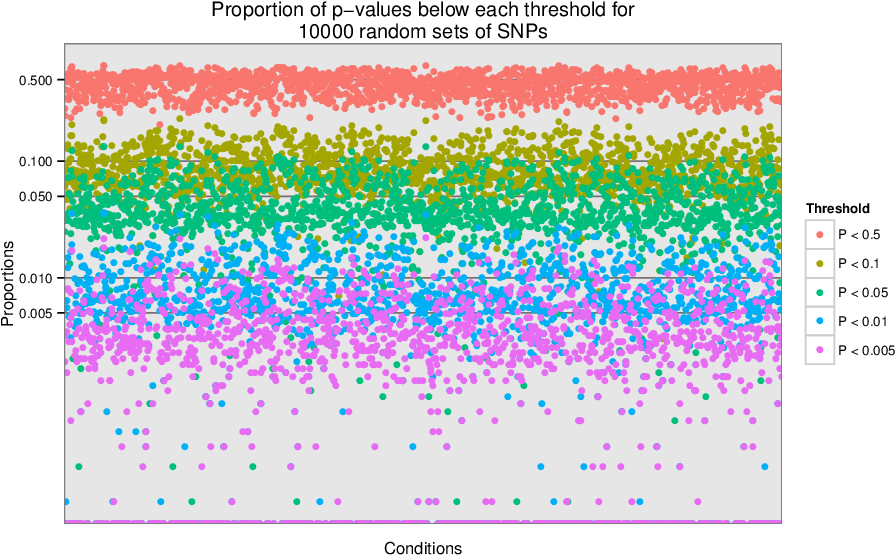
\includegraphics[width=0.85\textwidth]{figures/type1error_GO2013}\hfill{}

We sampled 10,000 sets of 100 SNPs uniformly from a list of LD-pruned
SNPs \cite{lango_allen_hundreds_2010}. We tested each of the 10,000
sets for enrichment of tissue-specific expression in the Gene Atlas
\cite{su_gene_2004} gene expression matrix (top) and for enrichment
of annotation with Gene Ontology terms (bottom). For each condition,
we show the proportion of the 10,000 enrichment p-values that are
below the given thresholds. We observe that the p-values are near
the expected values, so the type 1 (false positive) error rate is
well-calibrated.

\newpage{}


\section{Additional Examples}

We tested SNPsea with the three additional phenotypes listed below
with genome-wide significant SNPs $(P\leq5\times10^{-8})$. When multiple
SNPs implicated the same genes, we merged them into a single locus.
We tested each phenotype with the Gene Atlas and GO matrices with
the \texttt{'-{}-score single'} option. Below we show the number of
significantly enriched conditions we found for each phenotype.

\vspace*{\bigskipamount}


\hspace*{\fill}%
\begin{tabular}{lccccll}
 &  &  & \multicolumn{2}{c}{} & \multicolumn{2}{l}{}\tabularnewline
Phenotype & SNPs & Loci & GO & Gene Atlas & Reference & \tabularnewline
\hline 
Red blood cell count & 45 & 45 & 1 & 1 & Table 1 & van der Harst, \emph{et al.} 2012 \cite{van_der_harst_seventy-five_2012}\tabularnewline
Multiple sclerosis & 51 & 47 & 52 & 6 & Supp. Table A & IMSGC WTCCC 2011 \cite{the_international_multiple_sclerosis_genetics_consortium_&_the_wellcome_trust_case_control_consortium_genetic_2011}\tabularnewline
Celiac disease & 35 & 34 & 28 & 3 & Table 2 & Trynka, \emph{et al.} 2011 \cite{trynka_dense_2011}\tabularnewline
HDL cholesterol & 46 & 46 & 13 & 1 & Supp. Table 2 & Teslovich, \emph{et al.} 2010 \cite{teslovich_biological_2010}\tabularnewline
\end{tabular}\hspace*{\fill}

\newpage{}


\subsection{Supplementary Figure 6: Red blood cell count GO enrichment}

\hfill{}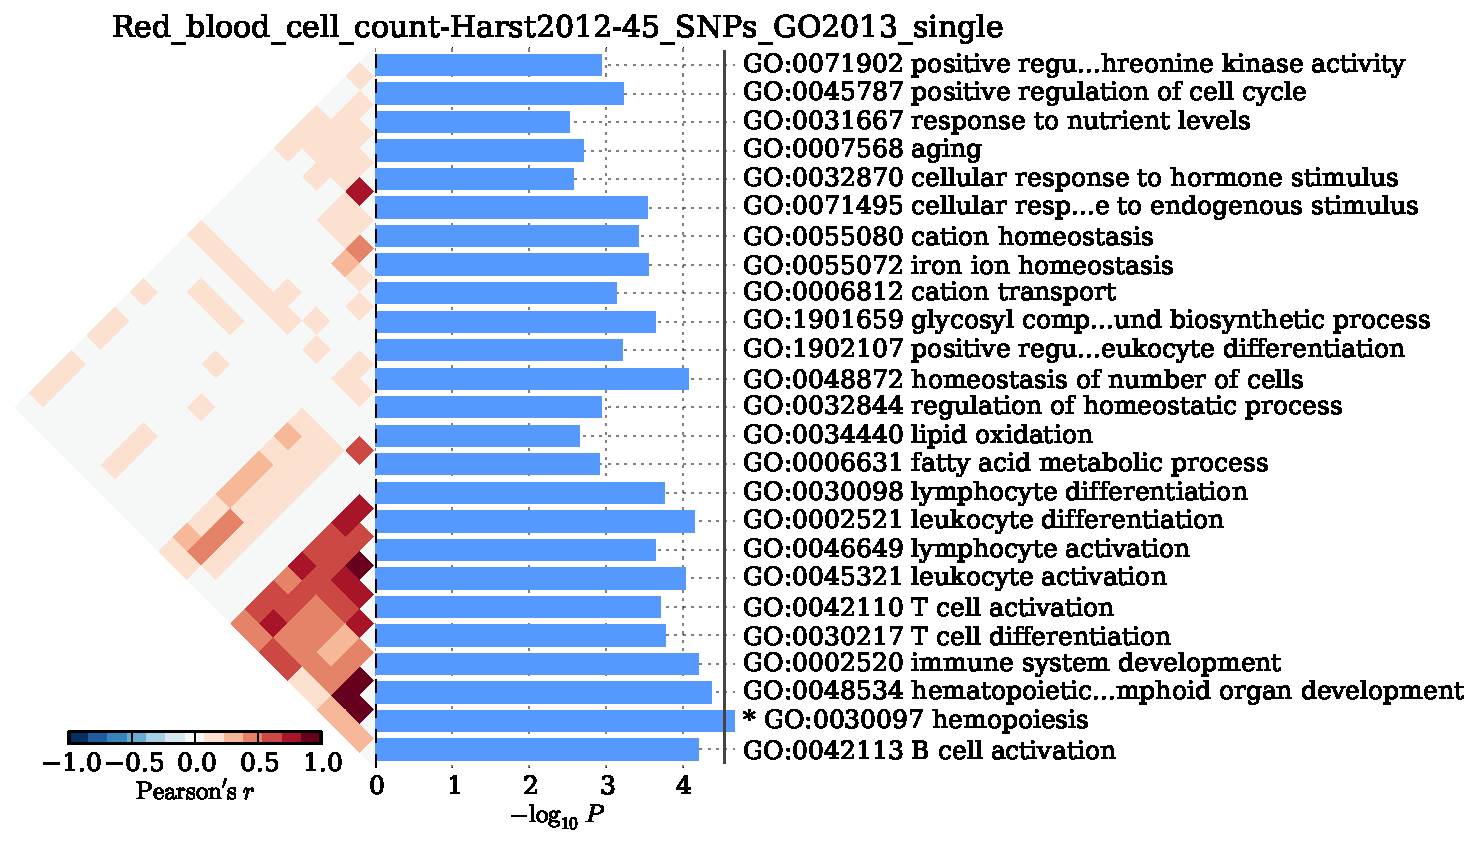
\includegraphics[width=1\textwidth]{figures/Red_blood_cell_count-Harst2012-45_SNPs-GO2013-single-pvalues_barplot}\hfill{}

We observed significant enrichment for \emph{hemopoiesis} $(2\times10^{-5})$.
The top 25 terms are shown.

\newpage{}


\subsection{Supplementary Figure 7: Multiple sclerosis}

\vfill{}


\hfill{}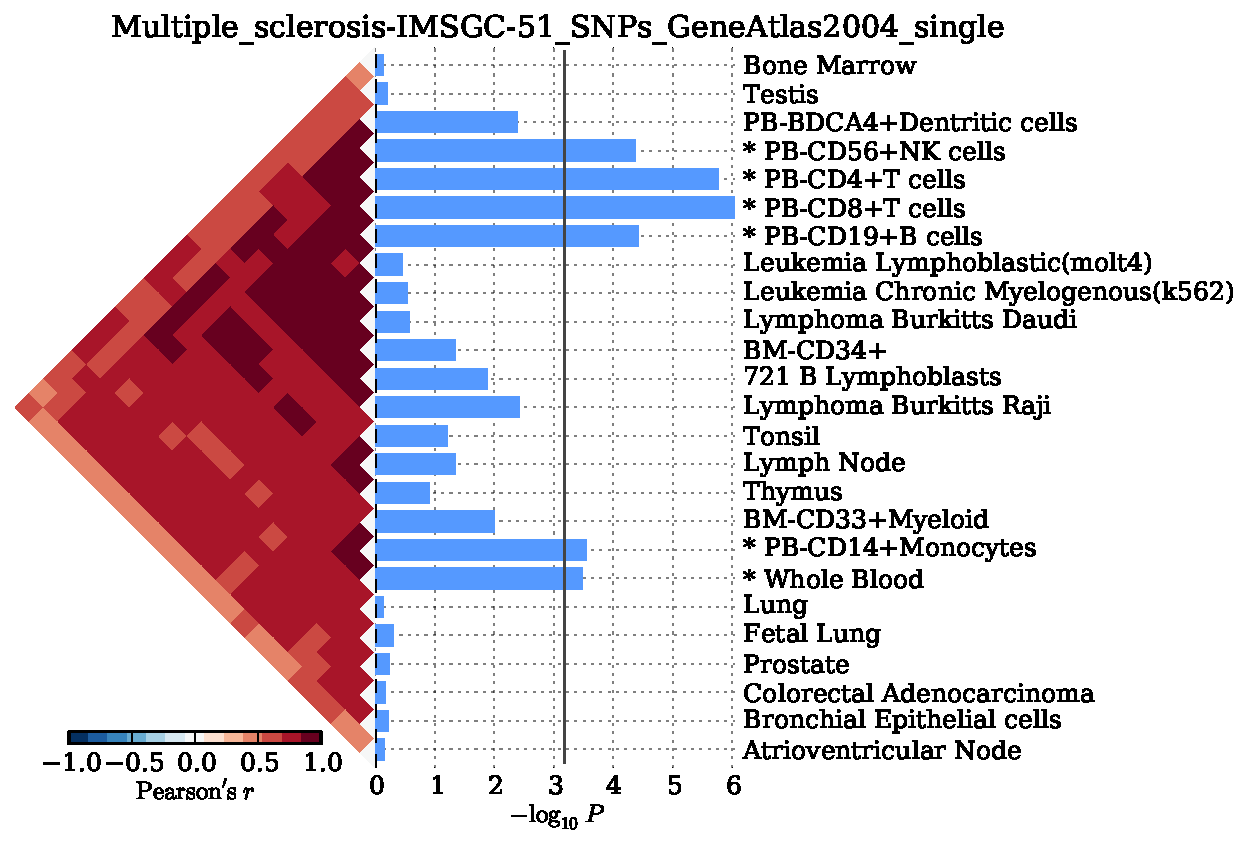
\includegraphics[width=0.65\textwidth]{figures/Multiple_sclerosis-IMSGC-51_SNPs-GeneAtlas2004-single-pvalues_barplot}\hfill{}

We observed significant enrichment for 6 cell types. The top 25 of
79 are shown.

\vfill{}


\hfill{}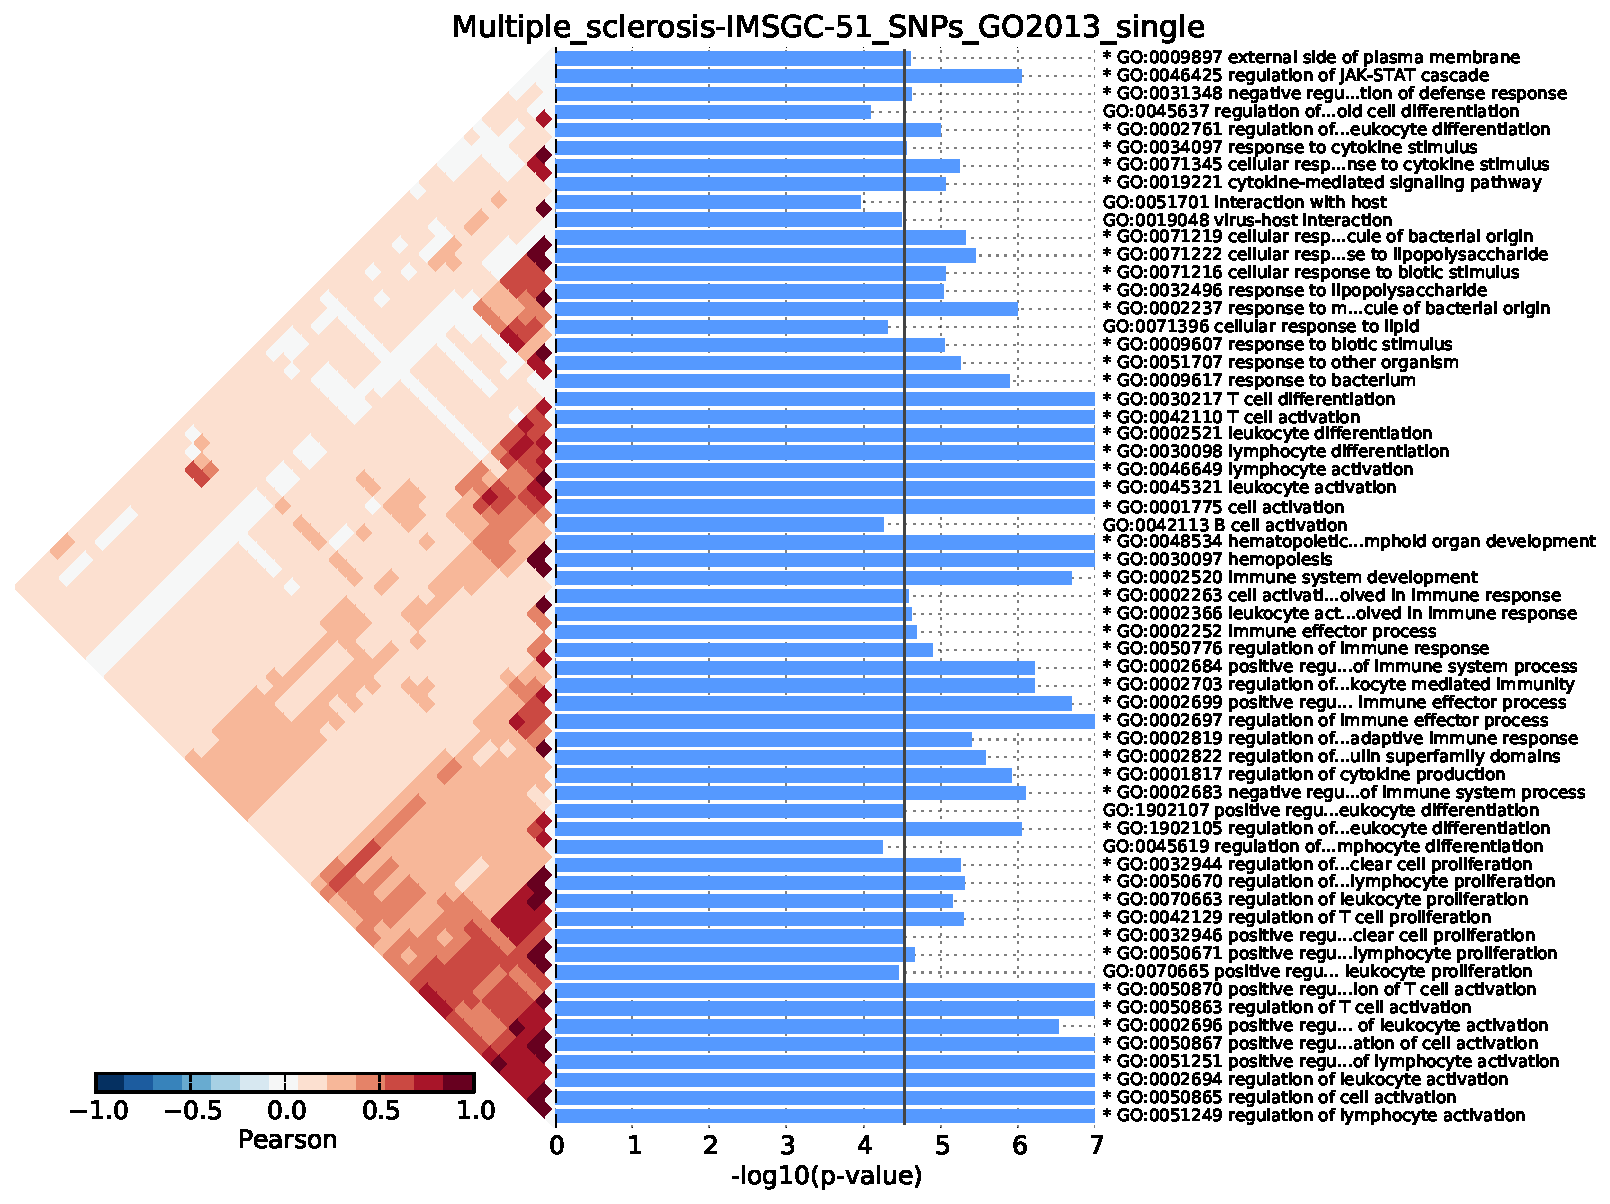
\includegraphics[width=0.95\textwidth]{figures/Multiple_sclerosis-IMSGC-51_SNPs-GO2013-single-pvalues_barplot}\hfill{}

We observed significant enrichment for 52 Gene Ontology terms. The
top 60 terms are shown.

\vfill{}


\newpage{}


\subsection{Supplementary Figure 8: Celiac disease}

\vfill{}


\hfill{}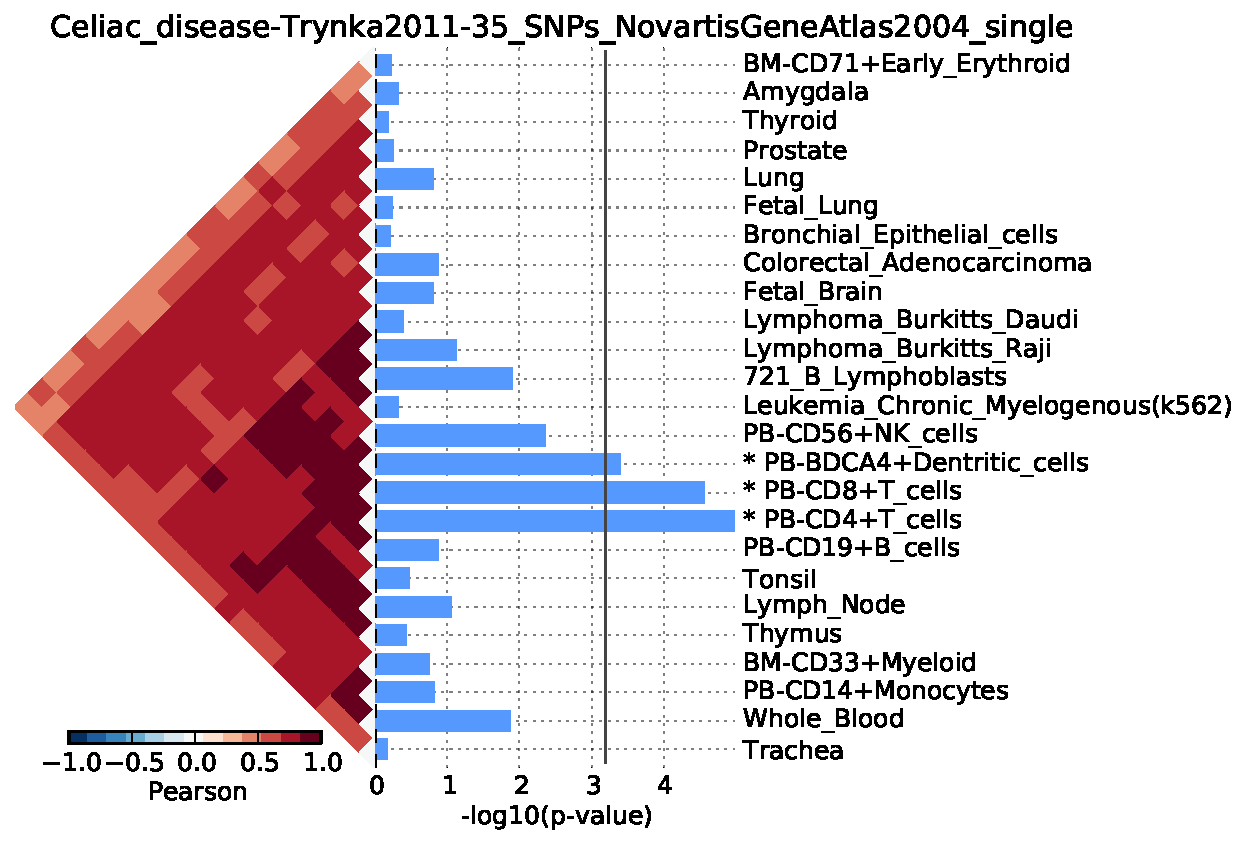
\includegraphics[width=0.65\textwidth]{figures/Celiac_disease-Trynka2011-35_SNPs-GeneAtlas2004-single-pvalues_barplot}\hfill{}

We observed significant enrichment for 3 cell types. The top 25 of
79 are shown.

\vfill{}


\hfill{}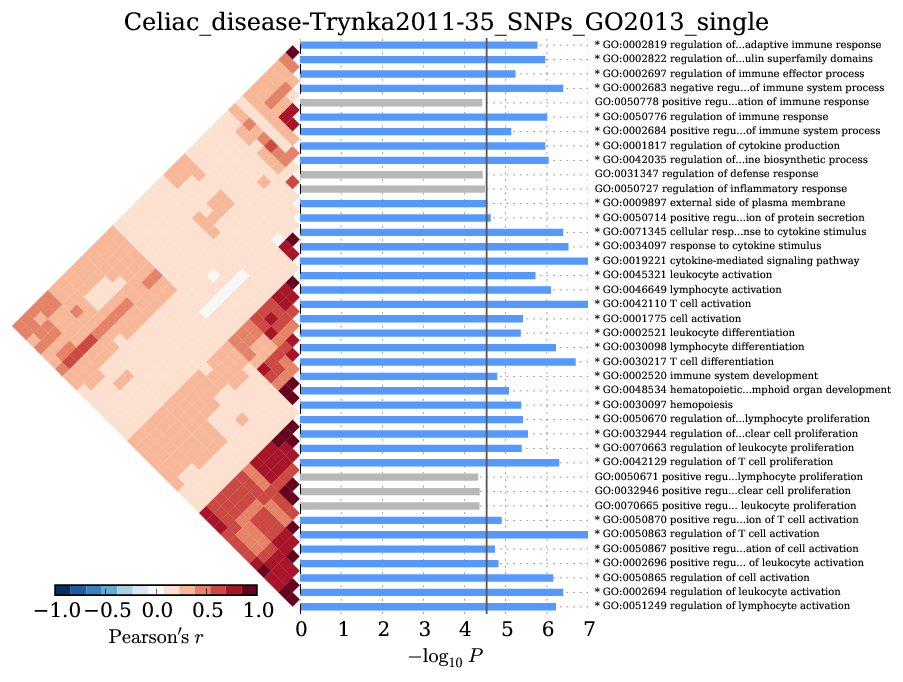
\includegraphics[width=1\textwidth]{figures/Celiac_disease-Trynka2011-35_SNPs-GO2013-single-pvalues_barplot}\hfill{}

We observed significant enrichment for 28 Gene Ontology terms. The
top 40 terms are shown.

\vfill{}


\newpage{}


\subsection{Supplementary Figure 9: HDL cholester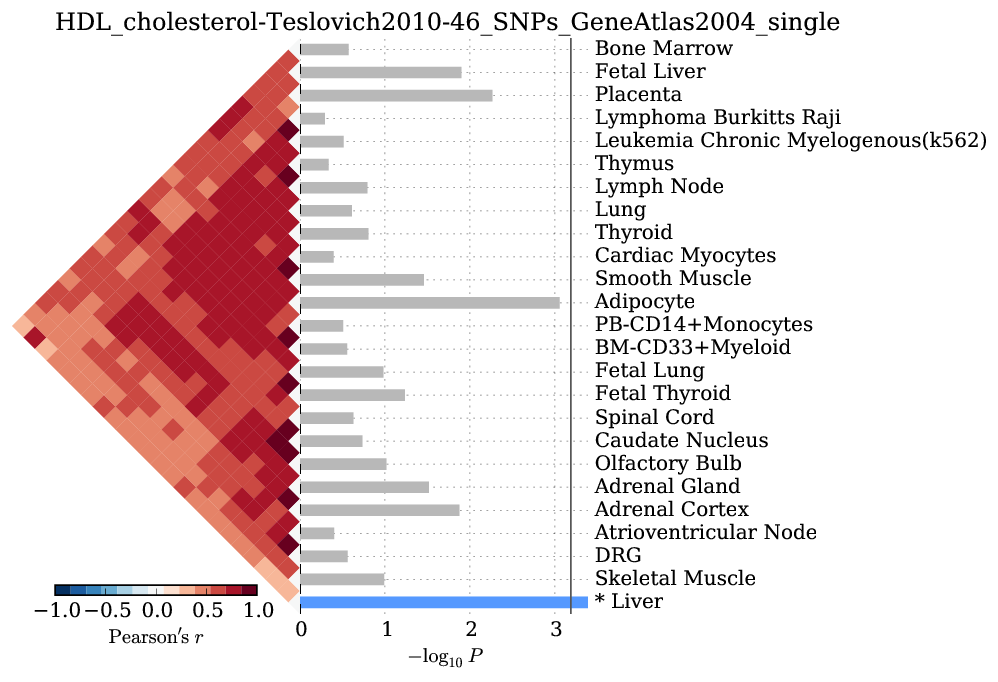
\includegraphics[width=1\includegraphics[width=0.65\textwidth]{figures/HDL_cholesterol-Teslovich2010-46_SNPs-GeneAtlas2004-single-pvalues_barplot}\hfill{}

We observed significant enrichment for liver tissue-specific gene
expression. The top 25 of 79 are shown.

\vfill{}


\hfill{}\includegraphics[width=0.8\textwidth]{figures/HDL_cholest\includegraphics[width=0.65\textwidth]{13_home_kamil_work_snpsea_

We observed significant enrichment for 13 Gene Ontology terms. The
top 25 term

We observed significant enrichment \bibliographystyle{unsrt}
\phantomsection\addcontentsline{toc}{section}{\refname}\bibliogra\includegraphics[width=0.8\textwidth]{14_home_kamil_work_snpsea_doc_figures_HDL_chole___h2010-46_SNPs-GO2013-single-pvalues_barplot.pdf}\hfill{}

We observed significant enrichment for 13 Gene Ontology terms. The
top 25 terms are shown.

\vfill{}


\newpage{}

